\section{Data Collection Details} \label{sec:collection_details}


\subsection{Data Preprocessing}

We downloaded the dump of English Wikipedia of October 1, 2017, and extracted text and hyperlinks with WikiExtractor.\footnote{\url{https://github.com/attardi/wikiextractor}}
 We use Stanford CoreNLP 3.8.0 \cite{manning-EtAl:2014:P14-5} for word and sentence tokenization.
 We use the resulting sentence boundaries for collection of supporting facts, and use token boundaries to check whether Turkers are providing answers that cover spans of entire tokens to avoid nonsensical partial-word answers.

\subsection{Further Data Collection Details}

\paragraph{Details on Curating Wikipedia Pages.}
To make sure the sampled candidate paragraph pairs are intuitive for crowd workers to ask high-quality multi-hop questions about, we manually curate 591 categories from the lists of popular pages by WikiProject.\footnote{\url{https://wiki.sh/y8qu}}
For each category, we sample $(a, b)$ pairs from the graph $G$ where $b$ is in the considered category, and manually check whether a multi-hop question can be asked given the pair $(a, b)$.
Those categories with a high probability of permitting multi-hop questions are selected.

\paragraph{Bonus Structures.} To incentivize crowd workers to produce higher-quality data more efficiently, we follow \citet{yang2017mastering}, and employ bonus structures. We mix two settings in our data collection process. In the first setting, we reward the top (in terms of numbers of examples) workers every 200 examples. In the second setting, the workers get bonuses based on their productivity (measured as the number of examples per hour).

\subsection{Crowd Worker Interface}

\begin{figure}
    \centering
    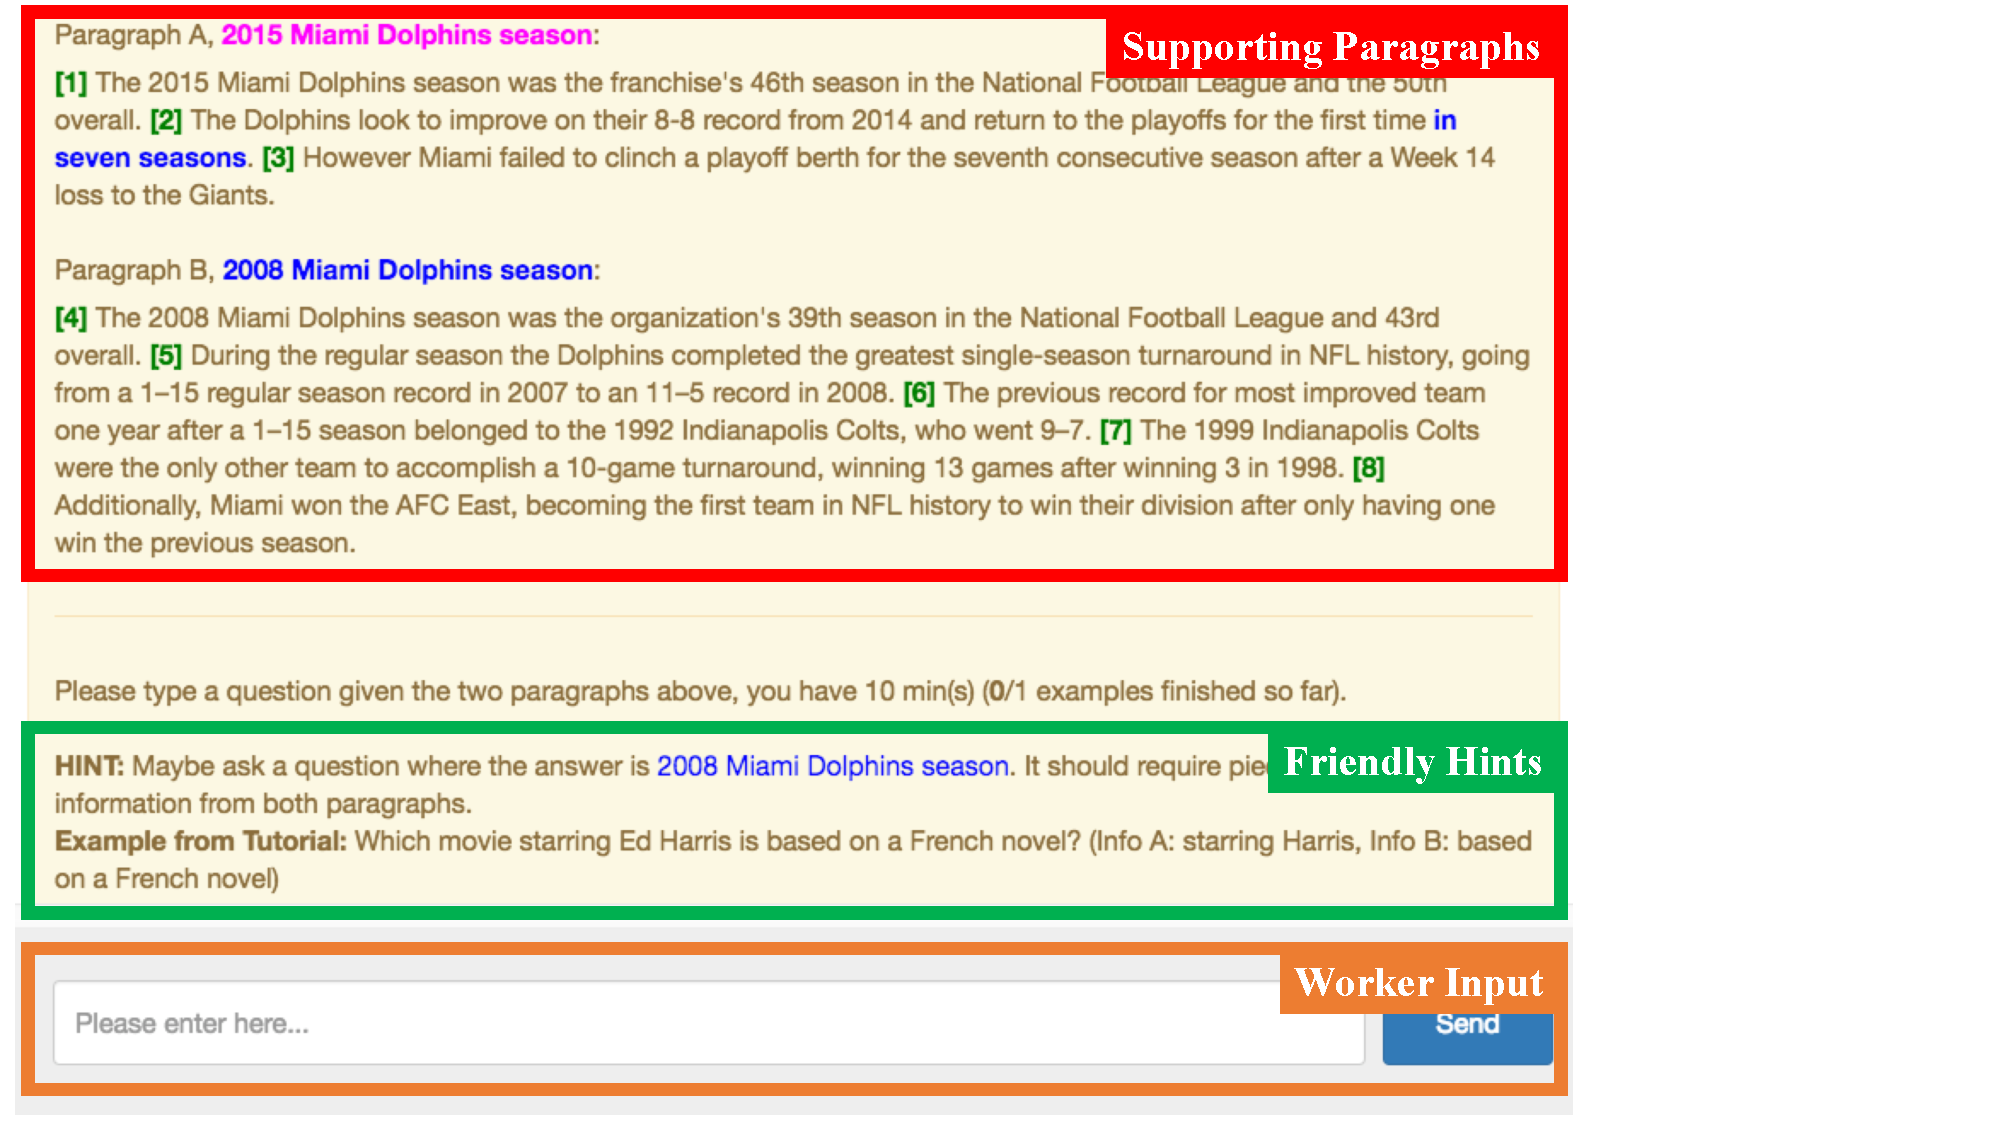
\includegraphics[width=.48\textwidth]{images/screenshot.pdf}
    \caption{Screenshot of our worker interface on Amazon Mechanical Turk.} \label{fig:interface}
\end{figure}

Our crowd worker interface is based on \parlai{} \cite{miller2017parlai}, an open-source project that facilitates the development of dialog systems and data collection with a dialog interface.
We adapt \parlai{} for collecting question answer pairs by converting the collection workflow into a system-oriented dialog.
This allows us to have more control over the turkers input, as well as provide turkers with in-the-loop feedbacks or helpful hints to help Turkers finish the task, and therefore speed up the collection process.

Please see Figure \ref{fig:interface} for an example of the worker interface during data collection.

\section{Further Data Analysis} \label{sec:further_analysis}

To further look into the diversity of the data in \datasetname{}, we further visualized the distribution of question lengths in the dataset in Figure \ref{fig:question_lengths}.
Besides being diverse in terms of types as is show in the main text, questions also vary greatly in length, indicating different levels of complexity and details covered.

\begin{figure}
    \centering
    \pgfplotstableread[row sep=\\,col sep=&]{
	l & count \\
	10	&	11506\\
	15	&	40554\\
	20	&	34054\\
	25	&	18523\\
	30	&	8858\\
	35	&	4398\\
	40	&	2356\\
	45	&	1535\\
	50	&	1074\\
	55	&	768\\
	60	&	607\\
	65	&	485\\
	70	&	321\\
	75	&	224\\
	80	&	141\\
	85	&	94\\
	90	&	49\\
	95	&	44\\
	100	&	22\\
	105	&	13\\
	110	&	3\\
	115	&	6\\
	120	&	6\\
	125	&	3\\
	130	&	1\\
}\mydata

\pgfplotsset{compat=1.8,
	/pgfplots/ybar legend/.style={
		/pgfplots/legend image code/.code={%
			%\draw[##1,/tikz/.cd,yshift=-0.25em]
			%(0cm,0cm) rectangle (3pt,0.8em);},
			\draw[##1,/tikz/.cd,bar width=3.5pt,yshift=-0.2em,bar shift=0pt]
			plot coordinates {(0cm,0.8em)};},
	},
}

\begin{tikzpicture}[font=\small]
\begin{axis}[
ybar=.5pt,
xtick={10, 30, 50, 70, 90, 110, 130},
ymin=0, ymax=45000,
ytick={1e4, 2e4, 3e4, 4e4},
xlabel={Question Length (tokens)},
ylabel={Number of Examples},
height=6.5cm,
/pgf/bar width=3.5pt,
xtick align=inside,
ymajorgrids=true,
grid style=dashed,
]

\addplot[draw opacity=0, fill=blue!50] table[x=l,y=count]{\mydata};

\end{axis}
\end{tikzpicture}
    \caption{Distribution of lengths of questions in \datasetname{}.} \label{fig:question_lengths}
\end{figure}

\section{Full Wiki Setting Details} \label{sec:fullwiki_details}
\subsection{The Inverted Index Filtering Strategy}

\begin{algorithm}
    \small
        \caption{Inverted Index Filtering Strategy}
        \label{algo:fullwiki_filter}
    \begin{algorithmic}
        \STATE {\bfseries Input:} question text $q$, control threshold $N$, ngram-to-Wikidoc inverted index $\mathcal{D}$
        \STATE {\bfseries Inintialize:}
            \STATE Extract unigram + bigram set $r_q$ from $q$
            \STATE $N_{cand} = +\infty$
            \STATE $C_{gram} = 0$
        \WHILE {$N_{cands} > N$}
            \STATE $C_{gram} = C_{gram} + 1$
            \STATE Set $S_{overlap}$ to be an empty dictionary
            \FOR {$w \in r_q$}
                 \FOR {$d \in \mathcal{D}[w]$}
                      \IF {$d$ not in $S_{overlap}$}
                           \STATE $S_{overlap}[d] = 1$
                      \ELSE
                           \STATE $S_{overlap}[d] = S_{overlap}[d] + 1$
                      \ENDIF
                 \ENDFOR
            \ENDFOR
            \STATE $S_{cand} = \emptyset$
            \FOR {$d$ in $S_{overlap}$}
                \IF {$S_{overlap}[d] \geq C_{gram}$}
                    \STATE $S_{cand} = S_{cand} \cup \{d\}$
                \ENDIF
            \ENDFOR
            \STATE $N_{cands} = |S_{cand}|$
        \ENDWHILE
        \RETURN $S_{cand}$
    \end{algorithmic}
    \end{algorithm}
In the full wiki setting, we adopt an efficient
inverted-index-based filtering strategy for preliminary
candidate paragraph retrieval. We provide details in Algorithm \ref{algo:fullwiki_filter}, where
we set the control threshold $N = 5000$ in our experiments.
For some of the question $q$, its corresponding gold paragraphs may not
be included in the output candidate pool $S_{cand}$,
we set such missing gold paragraph's rank as $|S_{cand}| + 1$ during the evaluation, so
MAP and Mean Rank reported in this paper are upper bounds of their true values.

\subsection{Compare \textit{train-medium} Split to Hard Ones}
Table \ref{tab:fullwiki_ir_train} shows the comparison between \textit{train-medium} split
and hard examples like \textit{dev} and \textit{test} under retrieval metrics in full wiki setting.
As we can see, the performance gap between \textit{train-medium} split and its
\textit{dev}/\textit{test} is close, which implies that \textit{train-medium} split has a similar level of
difficulty as hard examples under the full wiki setting in which a retrieval model is necessary as the first processing step.
\begin{table}[H]
    \small
    \centering
    \begin{tabular}{lcccc}
        \toprule
        Set & MAP & Mean Rank & CorAns Rank\\
        \midrule
        train-medium & 41.89 & 288.19 & 82.76 \\
        dev & 42.79 & 304.30 & 97.93  \\
        test & 45.92 & 286.20 & 74.85 \\
        \bottomrule
    \end{tabular}
    \caption{Retrieval performance comparison on full wiki setting for \textit{train-medium}, \textit{dev} and \textit{test} with 1,000 random samples each. MAP and are in \%. Mean Rank averages over retrieval ranks of two gold paragraphs. CorAns Rank refers to the rank of the gold paragraph containing the answer.} \label{tab:fullwiki_ir_train}
\end{table}
